\section{正則化と次元圧縮に関する実験の結果と考察}

図\ref{lasso}に,L1正則化を適用した正則化法と次元圧縮法のスコアの予測精度を示す.
図\ref{lasso}より,正則化法と次元圧縮法のスコア予測精度の違いは, MAEの中央値で$0.19 \sim 0.24$であることがわかる.
$10$段階評価での差であるので, $2$つの手法のスコア予測精度に差はないと考える.
L2正則化を適用した場合も同様の結果であった.
また,圧縮次元数とウィンドウサイズによるMAEに違いはないため,Word2Vecのハイパーパラメータはスコア予測精度に影響を与えないと考える.
しかし,圧縮次元数とウィンドウサイズを増やすに連れ実行時間が長くなるため,計算コストの観点では圧縮次元数とウィンドウサイズは小さいほうが良いといえる.

\begin{table}[t]
\begin{center}
\caption{正則化法と次元圧縮法のモデルの学習時間[s]}
  \begin{tabular}{c|c|cccc|c} \hline
      & \small 正則化法 & 次元圧縮法 \\ \hline
     \small L1正則化 & 34.2 & 23.6 \\
     \small L2正則化 & 77.4 & 23.4 \\  \hline
      \end{tabular}
      \label{jikkou}
      \end{center}
\end{table}

\begin{figure}[t]
  \centering
           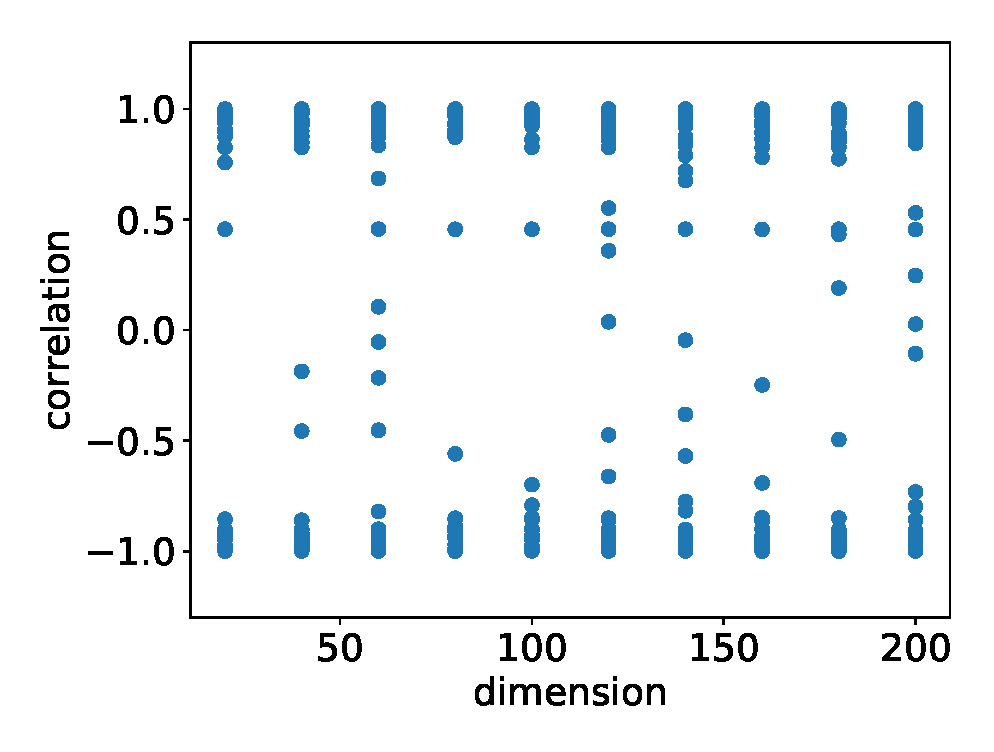
\includegraphics[width=0.8\hsize]{img/lasso-correlation-2.eps} \\
           \small ウィンドウサイズ2
        \caption{正則化法と次元圧縮法の偏回帰係数の相関(L1正則化)}
    \label{soukan}
%  \end{center}
\end{figure}
表\ref{jikkou}に, 正則化法と次元圧縮法について, $100$個の目的変数のモデル学習時間の合計を示す.
Word2Vecのハイパーパラメータは,圧縮次元数$20$次元,ウィンドウサイズ$2$に固定している.
表\ref{jikkou}より, $100$個の目的変数についてのモデル学習時間は次元圧縮法のほうが短いことがわかる.
目的変数$1$個あたりのモデル学習時間について考えると,本実験の環境下では目的変数の数$n$に対して実行時間$t$は$正則化法: t = 0.342 n, 次元圧縮法: t = 20.3 + 0.0330 n$のような$n$の1次式で表すことができる.
このことは,予測したい回帰式が多数ある場合は次元圧縮法のほうが低計算コストで学習できる事を示唆している.

図\ref{soukan}に,正則化法と次元圧縮法の偏回帰係数の相関の散布図を示す.
図\ref{soukan}より,圧縮次元数$20$次元,ウィンドウサイズ$2$の下では, 100個の回帰式のうち約$50$個には高い正の相関が,約$40$個には高い負の相関がみられる.
正則化法の偏回帰係数が正しいと仮定すると,次元圧縮法の偏回帰係数は必ずしも類似していないといえる.
現段階では,次元圧縮法での推薦の透明性の実現は難しいと考える.